\documentclass[11pt,a4paper]{article}

% Packages
\usepackage[utf8]{inputenc}
\usepackage[T1]{fontenc}
\usepackage{amsmath,amssymb,amsthm}
\usepackage{graphicx}
\usepackage{hyperref}
\usepackage{algorithm}
\usepackage{algpseudocode}
\usepackage{booktabs}
\usepackage{geometry}
\usepackage{xcolor}
\usepackage{tikz}
\usepackage{tcolorbox}
\usetikzlibrary{shapes,arrows,positioning,calc,decorations.pathreplacing}

\geometry{margin=1in}

% Custom commands
\newcommand{\ket}[1]{|#1\rangle}
\newcommand{\bra}[1]{\langle#1|}
\newcommand{\bigO}{\mathcal{O}}

% Custom boxes
\newtcolorbox{conceptbox}[1][]{colback=blue!5!white,colframe=blue!75!black,title=#1}
\newtcolorbox{keyinsight}[1][]{colback=green!5!white,colframe=green!75!black,title=#1}
\newtcolorbox{warningbox}[1][]{colback=red!5!white,colframe=red!75!black,title=#1}
\newtcolorbox{examplebox}[1][]{colback=yellow!5!white,colframe=yellow!75!black,title=#1}

\title{Belief Propagation for Quantum Error Correction:\\A Comprehensive Guide from Fundamentals to Advanced Techniques}

\author{Detailed Research Plan with Step-by-Step Explanations}

\date{\today}

\begin{document}

\maketitle

\begin{abstract}
This document provides a detailed, pedagogical introduction to belief propagation (BP) based quantum error correction schemes. Starting from the fundamental concepts of graphical models and message passing, we build up to advanced techniques including BP+OSD (Ordered Statistics Decoding), BP with Guided Decimation (BPGD), and the novel delayed-erasure BP algorithm. Each concept is explained slowly and thoroughly to ensure accessibility for readers new to the field. We conclude with a research roadmap for implementing BP-based decoders for atom loss errors in neutral atom quantum computers.
\end{abstract}

\tableofcontents
\newpage

%==============================================================================
\section{Introduction: Why Belief Propagation for Quantum Error Correction?}
%==============================================================================

Quantum error correction (QEC) is essential for building fault-tolerant quantum computers. The decoder is a critical component---it takes syndrome measurements (information about errors) and determines what correction to apply. The challenge is doing this \emph{fast} and \emph{accurately}.

\begin{keyinsight}[The Decoder Challenge]
A decoder must:
\begin{enumerate}
    \item Process syndrome data in real-time (often $<1\mu$s for superconducting qubits)
    \item Handle complex error patterns including correlations
    \item Scale to large codes with thousands of qubits
    \item Work reliably even under noisy conditions
\end{enumerate}
\end{keyinsight}

\textbf{Belief propagation} is a powerful algorithmic framework that addresses these challenges. Originally developed for classical error correction (LDPC codes), it has been adapted for quantum codes with remarkable success~\cite{roffe2020bp_osd}.

\subsection{What is Belief Propagation?}

At its core, belief propagation is a \emph{message-passing algorithm} that operates on graphical models. Think of it as a way for different parts of a system to ``communicate'' their beliefs about what happened, iteratively refining their estimates until they reach consensus~\cite{pearl1988bp}.

\begin{conceptbox}[Key Intuition]
Imagine you're trying to solve a puzzle where:
\begin{itemize}
    \item You have many variables (the error on each qubit)
    \item You have constraints (the syndrome measurements)
    \item Each constraint involves only a few variables
\end{itemize}
Belief propagation lets each constraint ``tell'' its variables what values are consistent with it, and each variable ``tells'' its constraints what values are likely given other constraints. Through iteration, a globally consistent solution emerges.
\end{conceptbox}

%==============================================================================
\section{Foundations: Graphical Models and the Tanner Graph}
%==============================================================================

Before diving into the algorithm, we need to understand the mathematical structure it operates on.

\subsection{What is a Graphical Model?}

A graphical model represents a probability distribution using a graph. The key idea is to express a complex joint probability distribution as a product of simpler \emph{factors}, each involving only a subset of variables~\cite{kschischang2001factorgraph}.

\begin{examplebox}[A Simple Example]
Suppose we have three binary variables $x_1, x_2, x_3$ with the joint probability:
\[
P(x_1, x_2, x_3) = \frac{1}{Z} f_a(x_1, x_2) \cdot f_b(x_2, x_3)
\]
where $f_a$ and $f_b$ are ``factor'' functions and $Z$ is a normalization constant.

This factors because:
\begin{itemize}
    \item $f_a$ only depends on $x_1$ and $x_2$
    \item $f_b$ only depends on $x_2$ and $x_3$
\end{itemize}

We can represent this as a \textbf{factor graph}:
\begin{center}
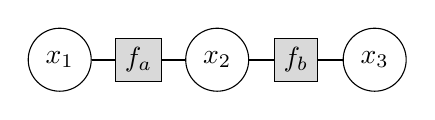
\begin{tikzpicture}[
    var/.style={circle, draw, fill=white, minimum size=0.8cm},
    factor/.style={rectangle, draw, fill=gray!30, minimum size=0.5cm},
    edge/.style={thick}
]
    \node[var] (x1) at (0,0) {$x_1$};
    \node[var] (x2) at (2,0) {$x_2$};
    \node[var] (x3) at (4,0) {$x_3$};

    \node[factor] (fa) at (1,0) {$f_a$};
    \node[factor] (fb) at (3,0) {$f_b$};

    \draw[edge] (x1) -- (fa);
    \draw[edge] (fa) -- (x2);
    \draw[edge] (x2) -- (fb);
    \draw[edge] (fb) -- (x3);
\end{tikzpicture}
\end{center}
Circles are \textbf{variable nodes}, squares are \textbf{factor nodes}.
\end{examplebox}

\subsection{The Tanner Graph for Error Correction}

For error correction codes, we use a special type of factor graph called a \textbf{Tanner graph}~\cite{tanner1981recursive}. Here:

\begin{itemize}
    \item \textbf{Variable nodes} represent potential error locations (one per qubit)
    \item \textbf{Check nodes} represent parity checks (syndrome measurements)
    \item An edge connects variable $v$ to check $c$ if qubit $v$ participates in check $c$
\end{itemize}

\begin{examplebox}[Tanner Graph for a Simple Code]
Consider a classical $[7,4,3]$ Hamming code with parity check matrix:
\[
H = \begin{pmatrix}
1 & 1 & 0 & 1 & 1 & 0 & 0 \\
1 & 0 & 1 & 1 & 0 & 1 & 0 \\
0 & 1 & 1 & 1 & 0 & 0 & 1
\end{pmatrix}
\]

The Tanner graph has:
\begin{itemize}
    \item 7 variable nodes (bits 1-7)
    \item 3 check nodes (rows of $H$)
    \item An edge from variable $j$ to check $i$ wherever $H_{ij} = 1$
\end{itemize}

\begin{center}
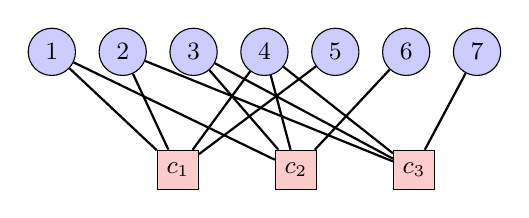
\begin{tikzpicture}[
    var/.style={circle, draw, fill=blue!20, minimum size=0.6cm, font=\small},
    check/.style={rectangle, draw, fill=red!20, minimum size=0.5cm, font=\small},
    edge/.style={thick}
]
    % Variable nodes
    \foreach \i in {1,...,7} {
        \node[var] (v\i) at (\i*0.9, 0) {\i};
    }

    % Check nodes
    \node[check] (c1) at (2.5, -1.5) {$c_1$};
    \node[check] (c2) at (4, -1.5) {$c_2$};
    \node[check] (c3) at (5.5, -1.5) {$c_3$};

    % Edges (based on H matrix)
    % c1: connects to 1,2,4,5
    \draw[edge] (v1) -- (c1);
    \draw[edge] (v2) -- (c1);
    \draw[edge] (v4) -- (c1);
    \draw[edge] (v5) -- (c1);

    % c2: connects to 1,3,4,6
    \draw[edge] (v1) -- (c2);
    \draw[edge] (v3) -- (c2);
    \draw[edge] (v4) -- (c2);
    \draw[edge] (v6) -- (c2);

    % c3: connects to 2,3,4,7
    \draw[edge] (v2) -- (c3);
    \draw[edge] (v3) -- (c3);
    \draw[edge] (v4) -- (c3);
    \draw[edge] (v7) -- (c3);
\end{tikzpicture}
\end{center}
\end{examplebox}

\subsection{Quantum Codes: The CSS Construction}

For quantum codes, the situation is more complex because we have two types of errors: \textbf{bit-flips} ($X$ errors) and \textbf{phase-flips} ($Z$ errors). CSS codes (Calderbank-Shor-Steane) handle this elegantly~\cite{calderbank1996css}:

\begin{itemize}
    \item $X$-type stabilizers detect $Z$ errors
    \item $Z$-type stabilizers detect $X$ errors
\end{itemize}

For a CSS code, we typically have two parity check matrices $H_X$ and $H_Z$, and correspondingly, two Tanner graphs that can be decoded (partially) independently.

\begin{keyinsight}[Quantum vs. Classical]
A key challenge in quantum decoding is \textbf{degeneracy}: multiple different physical error patterns can have the same syndrome and the same effect on the logical qubit. This is actually a \emph{feature}---it provides extra error tolerance---but it complicates decoding because BP doesn't naturally account for it~\cite{poulin2008mbp}.
\end{keyinsight}

%==============================================================================
\section{The Belief Propagation Algorithm: Step by Step}
%==============================================================================

Now let's understand how the algorithm actually works. We'll build it up piece by piece.

\subsection{The Basic Idea: Message Passing}

The algorithm works by passing \textbf{messages} along the edges of the Tanner graph. There are two types of messages:

\begin{enumerate}
    \item \textbf{Variable-to-check messages} ($\mu_{v \to c}$): Variable $v$ tells check $c$ its current belief about whether it has an error
    \item \textbf{Check-to-variable messages} ($\mu_{c \to v}$): Check $c$ tells variable $v$ what the check thinks about $v$'s error status, given what it knows about other variables
\end{enumerate}

\begin{center}
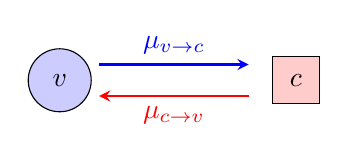
\begin{tikzpicture}[
    var/.style={circle, draw, fill=blue!20, minimum size=0.8cm},
    check/.style={rectangle, draw, fill=red!20, minimum size=0.6cm},
    arrow/.style={->, >=stealth, thick}
]
    \node[var] (v) at (0,0) {$v$};
    \node[check] (c) at (3,0) {$c$};

    \draw[arrow, blue] (0.5, 0.2) -- (2.4, 0.2) node[midway, above] {$\mu_{v \to c}$};
    \draw[arrow, red] (2.4, -0.2) -- (0.5, -0.2) node[midway, below] {$\mu_{c \to v}$};
\end{tikzpicture}
\end{center}

\subsection{Log-Likelihood Ratios (LLRs)}

Instead of working with probabilities directly, we use \textbf{log-likelihood ratios}:

\begin{equation}
\text{LLR}(v) = \log \frac{P(v = 0)}{P(v = 1)} = \log \frac{P(\text{no error})}{P(\text{error})}
\end{equation}

\begin{conceptbox}[Why LLRs?]
LLRs have several advantages:
\begin{itemize}
    \item \textbf{Sign encodes decision}: Positive LLR $\Rightarrow$ probably no error; Negative LLR $\Rightarrow$ probably error
    \item \textbf{Magnitude encodes confidence}: Larger $|\text{LLR}|$ means more certainty
    \item \textbf{Addition replaces multiplication}: Combining independent evidence is just addition
    \item \textbf{Numerical stability}: Avoids very small probabilities
\end{itemize}
\end{conceptbox}

For a qubit with physical error rate $p$, the initial (prior) LLR is:
\begin{equation}
\lambda_v^{(0)} = \log \frac{1-p}{p}
\end{equation}

For $p = 0.01$, this gives $\lambda_v^{(0)} \approx 4.6$, indicating high confidence in ``no error.''

\subsection{Message Update Rules}

The algorithm proceeds in rounds. In each round:

\subsubsection{Step 1: Variable-to-Check Messages}

Each variable node $v$ sends a message to each neighboring check $c$. The message represents $v$'s belief about itself, incorporating information from \emph{all other} checks except $c$:

\begin{equation}
\mu_{v \to c}^{(t)} = \lambda_v^{(0)} + \sum_{c' \in \mathcal{N}(v) \setminus \{c\}} \mu_{c' \to v}^{(t-1)}
\end{equation}

\begin{center}
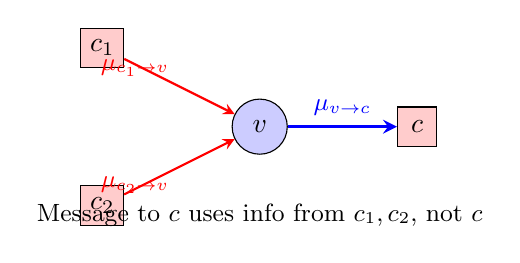
\begin{tikzpicture}[
    var/.style={circle, draw, fill=blue!20, minimum size=0.7cm},
    check/.style={rectangle, draw, fill=red!20, minimum size=0.5cm},
    arrow/.style={->, >=stealth, thick}
]
    \node[var] (v) at (2,0) {$v$};

    \node[check] (c1) at (0,1) {$c_1$};
    \node[check] (c2) at (0,-1) {$c_2$};
    \node[check] (c) at (4,0) {$c$};

    \draw[arrow, red] (c1) -- (v) node[midway, above left, font=\small] {$\mu_{c_1 \to v}$};
    \draw[arrow, red] (c2) -- (v) node[midway, below left, font=\small] {$\mu_{c_2 \to v}$};
    \draw[arrow, blue, very thick] (v) -- (c) node[midway, above, font=\small] {$\mu_{v \to c}$};

    \node[below=0.5cm of v, font=\small] {Message to $c$ uses info from $c_1, c_2$, not $c$};
\end{tikzpicture}
\end{center}

\textbf{Intuition}: ``Dear check $c$, based on my prior and what checks $c_1$ and $c_2$ told me, here's my current belief about whether I have an error.''

\subsubsection{Step 2: Check-to-Variable Messages}

Each check node $c$ sends a message to each neighboring variable $v$. This is more complex---the check must convey what it implies about $v$ given the syndrome bit $s_c$ and information from other variables:

\begin{equation}
\mu_{c \to v}^{(t)} = (-1)^{s_c} \cdot 2 \tanh^{-1} \left( \prod_{v' \in \mathcal{N}(c) \setminus \{v\}} \tanh\left(\frac{\mu_{v' \to c}^{(t)}}{2}\right) \right)
\end{equation}

\begin{warningbox}[The Mysterious Formula]
This formula looks intimidating, but it has a beautiful interpretation. The $\tanh$ transformation maps LLRs to a $[-1,1]$ scale where:
\begin{itemize}
    \item $+1$ means ``definitely no error''
    \item $-1$ means ``definitely error''
    \item $0$ means ``completely uncertain''
\end{itemize}

The product computes the parity of the likely error pattern on other variables. The $(-1)^{s_c}$ accounts for the observed syndrome.
\end{warningbox}

\begin{examplebox}[Concrete Example]
Suppose check $c$ has syndrome $s_c = 1$ (odd parity detected) and connects to variables $v_1, v_2, v_3$. We want to compute $\mu_{c \to v_1}$.

If the incoming messages suggest:
\begin{itemize}
    \item $v_2$: LLR = 3 (probably no error, $\tanh(1.5) \approx 0.905$)
    \item $v_3$: LLR = 4 (probably no error, $\tanh(2) \approx 0.964$)
\end{itemize}

Product: $0.905 \times 0.964 \approx 0.872$

Since $s_c = 1$ (odd parity), and $v_2, v_3$ probably have no errors, the check implies $v_1$ probably \emph{has} an error:

$\mu_{c \to v_1} = (-1)^1 \cdot 2\tanh^{-1}(0.872) \approx -2.7$ (negative = likely error)
\end{examplebox}

\subsection{Final Decision}

After $T$ iterations (or convergence), compute the final belief for each variable:

\begin{equation}
\lambda_v^{\text{final}} = \lambda_v^{(0)} + \sum_{c \in \mathcal{N}(v)} \mu_{c \to v}^{(T)}
\end{equation}

The decoding decision is:
\begin{equation}
\hat{e}_v = \begin{cases}
1 & \text{if } \lambda_v^{\text{final}} < 0 \\
0 & \text{if } \lambda_v^{\text{final}} \geq 0
\end{cases}
\end{equation}

\subsection{Complete Algorithm}

\begin{algorithm}[H]
\caption{Sum-Product Belief Propagation (BP)}
\begin{algorithmic}[1]
\Require Tanner graph $G = (V, C, E)$, syndrome $s$, prior error rates $\{p_v\}$, max iterations $T$
\Ensure Estimated error pattern $\hat{e}$

\State \textbf{// Initialization}
\For{each variable $v \in V$}
    \State $\lambda_v^{(0)} \gets \log((1-p_v)/p_v)$ \Comment{Prior LLR}
\EndFor
\For{each edge $(v,c) \in E$}
    \State $\mu_{v \to c}^{(0)} \gets \lambda_v^{(0)}$ \Comment{Initial messages}
\EndFor

\State \textbf{// Main iteration loop}
\For{$t = 1$ to $T$}
    \State \textbf{// Check-to-variable messages}
    \For{each check $c \in C$}
        \For{each $v \in \mathcal{N}(c)$}
            \State $\pi \gets \prod_{v' \in \mathcal{N}(c) \setminus \{v\}} \tanh(\mu_{v' \to c}^{(t-1)}/2)$
            \State $\mu_{c \to v}^{(t)} \gets (-1)^{s_c} \cdot 2 \tanh^{-1}(\pi)$
        \EndFor
    \EndFor

    \State \textbf{// Variable-to-check messages}
    \For{each variable $v \in V$}
        \For{each $c \in \mathcal{N}(v)$}
            \State $\mu_{v \to c}^{(t)} \gets \lambda_v^{(0)} + \sum_{c' \in \mathcal{N}(v) \setminus \{c\}} \mu_{c' \to v}^{(t)}$
        \EndFor
    \EndFor

    \State \textbf{// Check convergence}
    \If{messages have converged}
        \State \textbf{break}
    \EndIf
\EndFor

\State \textbf{// Final decision}
\For{each variable $v \in V$}
    \State $\lambda_v^{\text{final}} \gets \lambda_v^{(0)} + \sum_{c \in \mathcal{N}(v)} \mu_{c \to v}^{(T)}$
    \State $\hat{e}_v \gets [\lambda_v^{\text{final}} < 0]$ \Comment{1 if negative, 0 otherwise}
\EndFor

\State \Return $\hat{e}$
\end{algorithmic}
\end{algorithm}

\subsection{Complexity Analysis}

\begin{itemize}
    \item \textbf{Time}: $\bigO(T \cdot |E|)$ where $|E|$ is the number of edges
    \item \textbf{Space}: $\bigO(|E|)$ to store messages
    \item For LDPC codes with constant row/column weight: $|E| = \bigO(n)$
    \item Total: $\bigO(T \cdot n)$ --- \textbf{linear in code size!}
\end{itemize}

This is why BP is so attractive: it scales linearly while providing near-optimal decoding for many codes.

%==============================================================================
\section{The Quantum Challenge: Why BP Struggles with Quantum Codes}
%==============================================================================

While BP works beautifully for classical LDPC codes, quantum codes present unique challenges~\cite{poulin2008mbp, kuo2022exploiting}.

\subsection{Challenge 1: Short Cycles in the Tanner Graph}

BP is \emph{exact} on tree-structured graphs (no cycles). On graphs with cycles, it's an approximation that may not converge~\cite{pearl1988bp}.

\begin{warningbox}[The Cycle Problem]
Quantum stabilizer codes inherently have many short cycles in their Tanner graphs:
\begin{itemize}
    \item Surface codes have 4-cycles everywhere
    \item CSS codes have correlated $X$ and $Z$ check structures
    \item These cycles cause messages to ``echo back,'' leading to overconfident beliefs
\end{itemize}
\end{warningbox}

\begin{center}
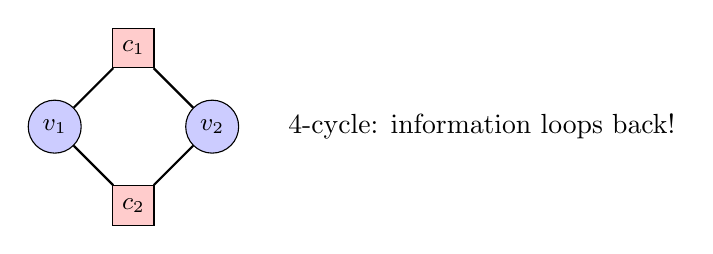
\begin{tikzpicture}[
    var/.style={circle, draw, fill=blue!20, minimum size=0.6cm, font=\small},
    check/.style={rectangle, draw, fill=red!20, minimum size=0.5cm, font=\small},
    edge/.style={thick}
]
    \node[var] (v1) at (0,0) {$v_1$};
    \node[var] (v2) at (2,0) {$v_2$};
    \node[check] (c1) at (1,1) {$c_1$};
    \node[check] (c2) at (1,-1) {$c_2$};

    \draw[edge] (v1) -- (c1);
    \draw[edge] (c1) -- (v2);
    \draw[edge] (v2) -- (c2);
    \draw[edge] (c2) -- (v1);

    \node[right=0.5cm of v2] {4-cycle: information loops back!};
\end{tikzpicture}
\end{center}

\subsection{Challenge 2: Degeneracy}

This is the deeper, more fundamental problem~\cite{kuo2022exploiting}.

\begin{conceptbox}[What is Degeneracy?]
Two error patterns $E_1$ and $E_2$ are \textbf{degenerate} if:
\begin{enumerate}
    \item They produce the same syndrome: $\sigma(E_1) = \sigma(E_2)$
    \item They have the same effect on logical information: $\bar{E}_1 = \bar{E}_2$
\end{enumerate}

The decoder doesn't need to identify the \emph{exact} physical error---it just needs to find an error in the same equivalence class.
\end{conceptbox}

\begin{examplebox}[Degeneracy Example]
Consider a distance-3 surface code. The following are degenerate:
\begin{itemize}
    \item Single $X$ error on qubit 5
    \item $X$ errors on qubits 5, 10, 11 (forming a stabilizer times the single error)
\end{itemize}
Both have the same syndrome and same logical effect. A smart decoder should recognize both as equally good solutions.
\end{examplebox}

\textbf{Why BP fails}: BP tries to find the \emph{most likely single error pattern}. It doesn't understand that degenerate patterns should be grouped together. When there are many degenerate options, BP gets ``confused'' and may converge to an incorrect solution or fail to converge at all.

\subsection{Symptoms of BP Failure on Quantum Codes}

\begin{enumerate}
    \item \textbf{Non-convergence}: Messages oscillate without settling
    \item \textbf{Incorrect hard decisions}: Even if soft outputs look reasonable, the hard decision is wrong
    \item \textbf{Poor syndrome matching}: The estimated error doesn't match the observed syndrome
\end{enumerate}

%==============================================================================
\section{Solutions: Advanced BP Techniques for Quantum Codes}
%==============================================================================

Researchers have developed several techniques to make BP work for quantum codes~\cite{roffe2020bp_osd, panteleev2021quantum}.

\subsection{Solution 1: BP + Ordered Statistics Decoding (BP+OSD)}

The most successful approach combines BP with a classical technique called OSD~\cite{roffe2020bp_osd}.

\begin{keyinsight}[The BP+OSD Strategy]
\begin{enumerate}
    \item Run BP to get soft information (beliefs) about each qubit
    \item Use BP's output to rank qubits by reliability
    \item Apply OSD: fix the most reliable qubits, solve for the rest using linear algebra
\end{enumerate}
\end{keyinsight}

\subsubsection{How OSD Works}

\begin{algorithm}[H]
\caption{Ordered Statistics Decoding (OSD) Post-Processing}
\begin{algorithmic}[1]
\Require BP soft outputs $\{\lambda_v\}$, parity check matrix $H$, syndrome $s$
\Ensure Corrected error estimate $\hat{e}$

\State \textbf{// Step 1: Sort qubits by reliability}
\State $\pi \gets \text{argsort}(|\lambda_v|)$ in \textbf{descending} order \Comment{Most reliable first}

\State \textbf{// Step 2: Permute $H$ according to reliability}
\State $H' \gets H$ with columns reordered by $\pi$

\State \textbf{// Step 3: Find most reliable independent set (MRI)}
\State Apply Gaussian elimination to find $H' = [I | P]$ (or closest form)
\State MRI $\gets$ indices of pivot columns (most reliable independent bits)

\State \textbf{// Step 4: Solve for MRI bits}
\State Set MRI bits to satisfy syndrome exactly using back-substitution

\State \textbf{// Step 5: (Optional) Search over non-MRI bits}
\For{each pattern $p$ of weight $\leq w$ on non-MRI bits}
    \State Compute corresponding MRI bits
    \State If total weight is lower, update solution
\EndFor

\State \Return best solution found
\end{algorithmic}
\end{algorithm}

\subsubsection{Why It Works}

\begin{itemize}
    \item BP provides good \emph{soft information} even when it doesn't converge
    \item The reliability ranking is usually correct even if hard decisions aren't
    \item OSD uses linear algebra to guarantee a valid syndrome-matching solution
    \item The combination handles degeneracy implicitly through the linear algebra
\end{itemize}

\subsubsection{Complexity}

\begin{itemize}
    \item BP phase: $\bigO(T \cdot n)$
    \item Gaussian elimination: $\bigO(n^2 \cdot m)$ or $\bigO(n^3)$
    \item OSD-$w$ search: $\bigO(\binom{n-m}{w})$ combinations
\end{itemize}

The OSD phase dominates, making BP+OSD slower than pure BP but still practical~\cite{roffe2020bp_osd}.

\subsection{Solution 2: BP with Guided Decimation (BPGD)}

An alternative that avoids the expensive OSD step~\cite{gokduman2024bpgd}.

\begin{keyinsight}[The BPGD Strategy]
Instead of running BP to completion and then post-processing:
\begin{enumerate}
    \item Run BP for a few iterations
    \item ``Decimate'': fix the most confident bit to its hard decision
    \item Repeat with the reduced problem
\end{enumerate}
\end{keyinsight}

\begin{algorithm}[H]
\caption{BP with Guided Decimation (BPGD)}
\begin{algorithmic}[1]
\Require Tanner graph $G$, syndrome $s$, parameters $T_{\text{BP}}, T_{\text{max}}$
\Ensure Estimated error $\hat{e}$

\State $\hat{e} \gets \mathbf{0}$ \Comment{Initialize all-zero error}
\State $U \gets V$ \Comment{Unfixed variables}

\For{$t = 1$ to $T_{\text{max}}$}
    \State \textbf{// Run BP on unfixed variables}
    \State $\{\lambda_v\}_{v \in U} \gets \textsc{BP}(G|_U, s', T_{\text{BP}})$

    \State \textbf{// Check if done}
    \If{syndrome is satisfied by current $\hat{e}$}
        \State \Return $\hat{e}$
    \EndIf

    \State \textbf{// Decimate: fix most confident variable}
    \State $v^* \gets \arg\max_{v \in U} |\lambda_v|$
    \State $\hat{e}_{v^*} \gets [\lambda_{v^*} < 0]$
    \State $U \gets U \setminus \{v^*\}$

    \State \textbf{// Update syndrome}
    \State $s' \gets$ syndrome remaining after accounting for $\hat{e}$
\EndFor

\State \Return $\hat{e}$
\end{algorithmic}
\end{algorithm}

\subsubsection{Advantages of BPGD}

\begin{itemize}
    \item \textbf{No linear algebra}: Avoids expensive Gaussian elimination
    \item \textbf{Escapes local optima}: Decimation prevents BP from getting stuck
    \item \textbf{Handles erasures naturally}: Known erasure locations can be decimated first
    \item \textbf{Parallelizable}: Each BP phase can be parallelized
\end{itemize}

\subsection{Solution 3: Memory-Based BP (MBP)}

Exploits degeneracy rather than fighting it~\cite{poulin2008mbp, kuo2022exploiting}.

\begin{conceptbox}[The MBP Idea]
Add ``memory'' to the BP updates: instead of using just the current messages, incorporate information from previous iterations. This acts like a damping mechanism that:
\begin{itemize}
    \item Prevents oscillation
    \item Allows exploration of degenerate solutions
    \item Functions similar to a neural network with recurrent connections
\end{itemize}
\end{conceptbox}

The update rule becomes:
\begin{equation}
\mu_{v \to c}^{(t)} = \alpha \cdot \mu_{v \to c}^{(t-1)} + (1-\alpha) \cdot \left[\lambda_v^{(0)} + \sum_{c' \neq c} \mu_{c' \to v}^{(t-1)}\right]
\end{equation}

where $\alpha \in [0,1)$ is the memory parameter.

\subsection{Solution 4: Restart Belief (RB)}

A recent technique that combines BP with a restart mechanism~\cite{valentini2025restart}.

\begin{keyinsight}[The Restart Mechanism]
When BP stalls (stops making progress):
\begin{enumerate}
    \item Identify which variables are ``stuck''
    \item Reset their beliefs to a perturbed state
    \item Continue BP from the new starting point
\end{enumerate}
This allows escaping local optima without the cost of OSD.
\end{keyinsight}

\subsection{Comparison of Techniques}

\begin{table}[h]
\centering
\caption{Comparison of BP-based decoders for quantum LDPC codes}
\begin{tabular}{lcccc}
\toprule
\textbf{Method} & \textbf{Accuracy} & \textbf{Speed} & \textbf{Complexity} & \textbf{Hardware-Friendly} \\
\midrule
Pure BP & Poor & Fast & $\bigO(Tn)$ & Yes \\
BP+OSD & Excellent & Slow & $\bigO(n^3)$ & No \\
BPGD & Good & Medium & $\bigO(Tn^2)$ & Partial \\
MBP & Good & Fast & $\bigO(Tn)$ & Yes \\
RB & Very Good & Medium & $\bigO(Tn)$ & Yes \\
\bottomrule
\end{tabular}
\end{table}

%==============================================================================
\section{Extension to Delayed-Erasure Decoding}
%==============================================================================

This section connects to the novel research direction from the companion report on atom loss decoding.

\subsection{The Delayed-Erasure Problem}

In neutral atom quantum computers:
\begin{itemize}
    \item Atoms can be \textbf{lost} from the trap during computation
    \item Loss is detected at measurement (delayed detection)
    \item The \textbf{when} and \textbf{where} the loss occurred is uncertain
    \item Loss creates a ``lifecycle'' of possible error locations
\end{itemize}

\begin{examplebox}[Lifecycle Example]
An atom measured as lost at time $T$ might have been lost:
\begin{itemize}
    \item After gate 1 with probability $p_1$ (causing error $E_1$)
    \item After gate 2 with probability $p_2$ (causing error $E_2$)
    \item After gate 3 with probability $p_3$ (causing error $E_3$)
    \item ...
\end{itemize}

The decoder must marginalize over these possibilities!
\end{examplebox}

\subsection{Lifecycle-Marginalized BP}

The key innovation is modifying BP to incorporate lifecycle uncertainty:

\begin{algorithm}[H]
\caption{Delayed-Erasure BP (DE-BP) - Key Modification}
\begin{algorithmic}[1]
\Require Lost qubit $i$ with lifecycle $\mathcal{L}_i = \{(t_1, p_1), \ldots, (t_k, p_k)\}$

\State \textbf{// Compute marginalized prior for variable $v$ affected by loss}
\State $\lambda_v^{\text{loss}} \gets 0$

\For{each loss time $(t_j, p_j) \in \mathcal{L}_i$}
    \If{$v$ is in the induced error set for loss at $t_j$}
        \State $w_j \gets \text{conditional probability of loss at } t_j$
        \State $\lambda_v^{\text{loss}} \gets \textsc{LogSumExp}(\lambda_v^{\text{loss}}, \log(w_j))$
    \EndIf
\EndFor

\State \textbf{// Combine with standard prior}
\State $\lambda_v^{(0)} \gets \textsc{LogSumExp}(\lambda_v^{\text{Pauli}}, \lambda_v^{\text{loss}})$
\end{algorithmic}
\end{algorithm}

\begin{keyinsight}[Why This Works]
By folding the lifecycle uncertainty into the prior probabilities, we enable standard BP to implicitly consider all possible loss locations. The marginalization is done once at initialization, so the BP iterations themselves are unchanged.
\end{keyinsight}

\subsection{Handling Invalid Checks}

When atoms are lost, some stabilizer measurements become invalid (they involve a missing qubit). The decoder must:

\begin{enumerate}
    \item Identify which checks are affected by loss
    \item Either remove these checks from the graph, or
    \item Create ``superchecks'' by combining adjacent valid checks
\end{enumerate}

This is detailed in the Baranes et al. delayed-erasure framework~\cite{baranes2025leveraging}.

%==============================================================================
\section{Hardware Implementation Considerations}
%==============================================================================

For practical quantum computers, decoders must run in real-time on specialized hardware~\cite{riverlane2024, fpga_bp_osd2025}.

\subsection{FPGA Implementation of BP}

\begin{keyinsight}[Why FPGAs for BP?]
\begin{itemize}
    \item \textbf{Parallelism}: All messages in one direction can update simultaneously
    \item \textbf{Fixed-point}: LLRs can be represented in few bits (6-8 typical)
    \item \textbf{Deterministic latency}: Important for real-time QEC
    \item \textbf{Low power}: Critical for cryogenic environments
\end{itemize}
\end{keyinsight}

\subsubsection{Architecture Overview}

\begin{center}
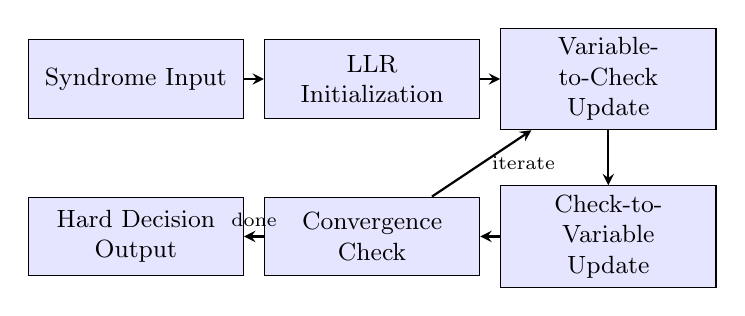
\begin{tikzpicture}[
    block/.style={rectangle, draw, fill=blue!10, text width=2.5cm, text centered, minimum height=1cm, font=\small},
    arrow/.style={->, >=stealth, thick}
]
    \node[block] (input) at (0,0) {Syndrome Input};
    \node[block] (init) at (3,0) {LLR\\Initialization};
    \node[block] (v2c) at (6,0) {Variable-to-Check\\Update};
    \node[block] (c2v) at (6,-2) {Check-to-Variable\\Update};
    \node[block] (conv) at (3,-2) {Convergence\\Check};
    \node[block] (out) at (0,-2) {Hard Decision\\Output};

    \draw[arrow] (input) -- (init);
    \draw[arrow] (init) -- (v2c);
    \draw[arrow] (v2c) -- (c2v);
    \draw[arrow] (c2v) -- (conv);
    \draw[arrow] (conv) -- (v2c) node[midway, right, font=\scriptsize] {iterate};
    \draw[arrow] (conv) -- (out) node[midway, above, font=\scriptsize] {done};
\end{tikzpicture}
\end{center}

\subsubsection{Recent Results}

From recent research on BP+OSD FPGA/ASIC implementations~\cite{fpga_bp_osd2025}:
\begin{itemize}
    \item Surface codes up to distance 9 fit on single VCU129 FPGA
    \item Maximum frequency: 200 MHz
    \item Worst-case latency: 134 $\mu$s
    \item For neutral atoms (4.5ms cycle time), this is more than sufficient
\end{itemize}

\subsection{Latency Budget for Neutral Atoms}

\begin{table}[h]
\centering
\caption{Latency comparison for different quantum platforms}
\begin{tabular}{lcc}
\toprule
\textbf{Platform} & \textbf{QEC Cycle Time} & \textbf{Available for Decoding} \\
\midrule
Superconducting & $\sim$1 $\mu$s & $<$ 1 $\mu$s \\
Trapped ions & $\sim$100 $\mu$s & $\sim$50 $\mu$s \\
Neutral atoms & $\sim$4.5 ms & $\sim$4 ms \\
\bottomrule
\end{tabular}
\end{table}

\begin{keyinsight}[The Neutral Atom Advantage]
Neutral atoms have 1000$\times$ more time for decoding than superconducting qubits. This allows:
\begin{itemize}
    \item More BP iterations
    \item OSD post-processing
    \item Complex lifecycle marginalization
    \item Even neural network inference
\end{itemize}
\end{keyinsight}

%==============================================================================
\section{Research Roadmap: Implementing BP for Atom Loss}
%==============================================================================

Based on the analysis above and the companion report, here is a concrete research plan.

\subsection{Phase 1: Foundation (Months 1-3)}

\begin{enumerate}
    \item \textbf{Implement standard BP decoder}
    \begin{itemize}
        \item Start with surface code Tanner graph
        \item Implement sum-product in LLR domain
        \item Validate against known results
    \end{itemize}

    \item \textbf{Add OSD post-processing}
    \begin{itemize}
        \item Implement Gaussian elimination for parity check matrix
        \item Add OSD-0 (zero additional search)
        \item Benchmark accuracy vs. pure BP
    \end{itemize}

    \item \textbf{Implement BPGD variant}
    \begin{itemize}
        \item Add decimation logic
        \item Compare with BP+OSD on accuracy and speed
    \end{itemize}
\end{enumerate}

\subsection{Phase 2: Erasure Extension (Months 4-6)}

\begin{enumerate}
    \item \textbf{Handle known erasures}
    \begin{itemize}
        \item Modify Tanner graph for erased qubits
        \item Update priors for erasure locations
        \item Validate against Perrin et al. results~\cite{perrin2024loss}
    \end{itemize}

    \item \textbf{Implement delayed-erasure marginalization}
    \begin{itemize}
        \item Build lifecycle data structures
        \item Compute marginalized priors
        \item Integrate with BP loop
    \end{itemize}

    \item \textbf{Supercheck construction}
    \begin{itemize}
        \item Implement algorithm to combine invalid checks
        \item Handle edge cases (multiple adjacent losses)
    \end{itemize}
\end{enumerate}

\subsection{Phase 3: Optimization (Months 7-9)}

\begin{enumerate}
    \item \textbf{Performance tuning}
    \begin{itemize}
        \item Profile bottlenecks
        \item Optimize memory access patterns
        \item Implement parallel updates
    \end{itemize}

    \item \textbf{Fixed-point implementation}
    \begin{itemize}
        \item Convert to fixed-point arithmetic
        \item Determine required precision
        \item Validate accuracy
    \end{itemize}

    \item \textbf{Template precomputation}
    \begin{itemize}
        \item Precompute lifecycle configurations
        \item Build lookup tables for common patterns
    \end{itemize}
\end{enumerate}

\subsection{Phase 4: Hardware (Months 10-12)}

\begin{enumerate}
    \item \textbf{FPGA prototype}
    \begin{itemize}
        \item Port BP core to Verilog/VHDL
        \item Implement pipelined architecture
        \item Target Xilinx VCU129 or similar
    \end{itemize}

    \item \textbf{Integration}
    \begin{itemize}
        \item Interface with syndrome input
        \item Add lifecycle lookup module
        \item Measure end-to-end latency
    \end{itemize}

    \item \textbf{Benchmarking}
    \begin{itemize}
        \item Compare with existing decoders (UF, MWPM)
        \item Measure logical error rate vs. physical error rate
        \item Validate meets timing requirements
    \end{itemize}
\end{enumerate}

%==============================================================================
\section{Conclusion}
%==============================================================================

Belief propagation offers a powerful framework for quantum error correction with several key advantages:

\begin{enumerate}
    \item \textbf{Linear complexity}: Scales well to large codes
    \item \textbf{Parallelizable}: Natural fit for FPGA/ASIC implementation
    \item \textbf{Flexible}: Can handle non-uniform error models through priors
    \item \textbf{Extensible}: Techniques like OSD, BPGD, and MBP address quantum-specific challenges
\end{enumerate}

For delayed-erasure decoding in neutral atom systems, BP is particularly promising because:
\begin{itemize}
    \item Lifecycle uncertainty naturally fits into the prior probability framework
    \item The longer QEC cycle times allow for more sophisticated post-processing
    \item The algorithm can be adapted incrementally from existing implementations
\end{itemize}

The research directions outlined in this document and the companion report provide a concrete path toward practical, high-performance decoders for the next generation of quantum computers.

%==============================================================================
% References
%==============================================================================

\bibliographystyle{unsrt}
\begin{thebibliography}{99}

\bibitem{pearl1988bp}
J.~Pearl.
\newblock Probabilistic Reasoning in Intelligent Systems: Networks of Plausible Inference.
\newblock Morgan Kaufmann, 1988.

\bibitem{kschischang2001factorgraph}
F.~R.~Kschischang, B.~J.~Frey, and H.-A.~Loeliger.
\newblock Factor graphs and the sum-product algorithm.
\newblock {\em IEEE Transactions on Information Theory}, 47(2):498--519, 2001.
\newblock \url{https://ieeexplore.ieee.org/document/910572/}

\bibitem{tanner1981recursive}
R.~M.~Tanner.
\newblock A recursive approach to low complexity codes.
\newblock {\em IEEE Transactions on Information Theory}, 27(5):533--547, 1981.

\bibitem{calderbank1996css}
A.~R.~Calderbank and P.~W.~Shor.
\newblock Good quantum error-correcting codes exist.
\newblock {\em Physical Review A}, 54(2):1098, 1996.

\bibitem{poulin2008mbp}
D.~Poulin and Y.~Chung.
\newblock On the iterative decoding of sparse quantum codes.
\newblock {\em Quantum Information and Computation}, 8(10):987--1000, 2008.

\bibitem{roffe2020bp_osd}
J.~Roffe, D.~R.~White, S.~Burton, and E.~T.~Campbell.
\newblock Decoding across the quantum low-density parity-check code landscape.
\newblock {\em Physical Review Research}, 2(4):043423, 2020.
\newblock \url{https://github.com/quantumgizmos/bp_osd}

\bibitem{panteleev2021quantum}
P.~Panteleev and G.~Kalachev.
\newblock Quantum LDPC codes with almost linear minimum distance.
\newblock {\em IEEE Transactions on Information Theory}, 68(1):213--229, 2021.

\bibitem{gokduman2024bpgd}
M.~G\"{o}kduman et al.
\newblock Belief propagation decoding of quantum LDPC codes with guided decimation.
\newblock {\em arXiv:2312.10950}, 2024.
\newblock \url{https://arxiv.org/abs/2312.10950}

\bibitem{kuo2022exploiting}
K.-Y.~Kuo and C.-Y.~Lai.
\newblock Exploiting degeneracy in belief propagation decoding of quantum codes.
\newblock {\em npj Quantum Information}, 8:111, 2022.
\newblock \url{https://www.nature.com/articles/s41534-022-00623-2}

\bibitem{valentini2025restart}
L.~Valentini, D.~Forlivesi, A.~Talarico, and M.~Chiani.
\newblock Restart belief: A general quantum LDPC decoder.
\newblock {\em arXiv:2511.13281}, 2025.
\newblock \url{https://arxiv.org/abs/2511.13281}

\bibitem{kwak2025evolutionary}
H.-Y.~Kwak et al.
\newblock Evolutionary BP+OSD decoding for low-latency quantum error correction.
\newblock {\em arXiv:2512.18273}, 2025.
\newblock \url{https://arxiv.org/abs/2512.18273}

\bibitem{fpga_bp_osd2025}
Exploring the FPGA and ASIC design space of belief propagation and ordered statistics decoders for quantum error correction codes.
\newblock {\em EPJ Quantum Technology}, 2025.
\newblock \url{https://link.springer.com/article/10.1140/epjqt/s40507-025-00446-y}

\bibitem{improved_bp2025}
Improved belief propagation decoding algorithms for surface codes.
\newblock {\em IEEE Transactions on Quantum Engineering}, 2025.
\newblock \url{https://tqe.ieee.org/2025/06/06/improved-belief-propagation-decoding-algorithms-for-surface-codes/}

\bibitem{pennylane_bp2025}
Decoding quantum errors on the Steane code with belief propagation \& Catalyst.
\newblock PennyLane Demos, 2025.
\newblock \url{https://pennylane.ai/qml/demos/tutorial_bp_catalyst}

\bibitem{riverlane2024}
Riverlane.
\newblock A real-time, scalable, fast decoder for quantum computers.
\newblock {\em Nature Electronics}, 2024.

\bibitem{perrin2024loss}
H.~Perrin et al.
\newblock Quantum error correction resilient against atom loss.
\newblock {\em Quantum}, 2025.
\newblock arXiv:2412.07841.

\bibitem{baranes2025leveraging}
G.~Baranes et al.
\newblock Leveraging atom loss errors in fault tolerant quantum algorithms.
\newblock {\em arXiv:2502.20558}, 2025.

\bibitem{accelerating_bp_osd2025}
Accelerating BP-OSD decoder for QLDPC codes with local syndrome-based preprocessing.
\newblock {\em arXiv:2509.01892}, 2025.
\newblock \url{https://arxiv.org/abs/2509.01892}

\bibitem{localized_statistics2025}
Localized statistics decoding for quantum low-density parity-check codes.
\newblock {\em Nature Communications}, 2025.
\newblock \url{https://pmc.ncbi.nlm.nih.gov/articles/PMC12405505/}

\end{thebibliography}

\end{document}
